
%%%%%%%%%%

\begin{frame}{\vskip -0.2cm \large The optimization problem behind classification trees}

\large
\begin{itemize}
\item
	{\Large Domain of objective function} {\small (a.k.a. hypothesis class)}
	{\scriptsize\begin{equation*}
	\left\{\begin{array}{c}
		\overset{{\color{white}.}}{\textnormal{recursive}} \\
		\textnormal{binary trees}
	\end{array}\right\}
	\quad\sim\quad
	\left\{\begin{array}{c}
		\overset{{\color{white}.}}{\textnormal{piecewise constant functions}} \\
		\textnormal{resulting from} \\
		\textnormal{recursive binary partitioning}
	\end{array}\right\}
	\end{equation*}}
	\begin{center}
	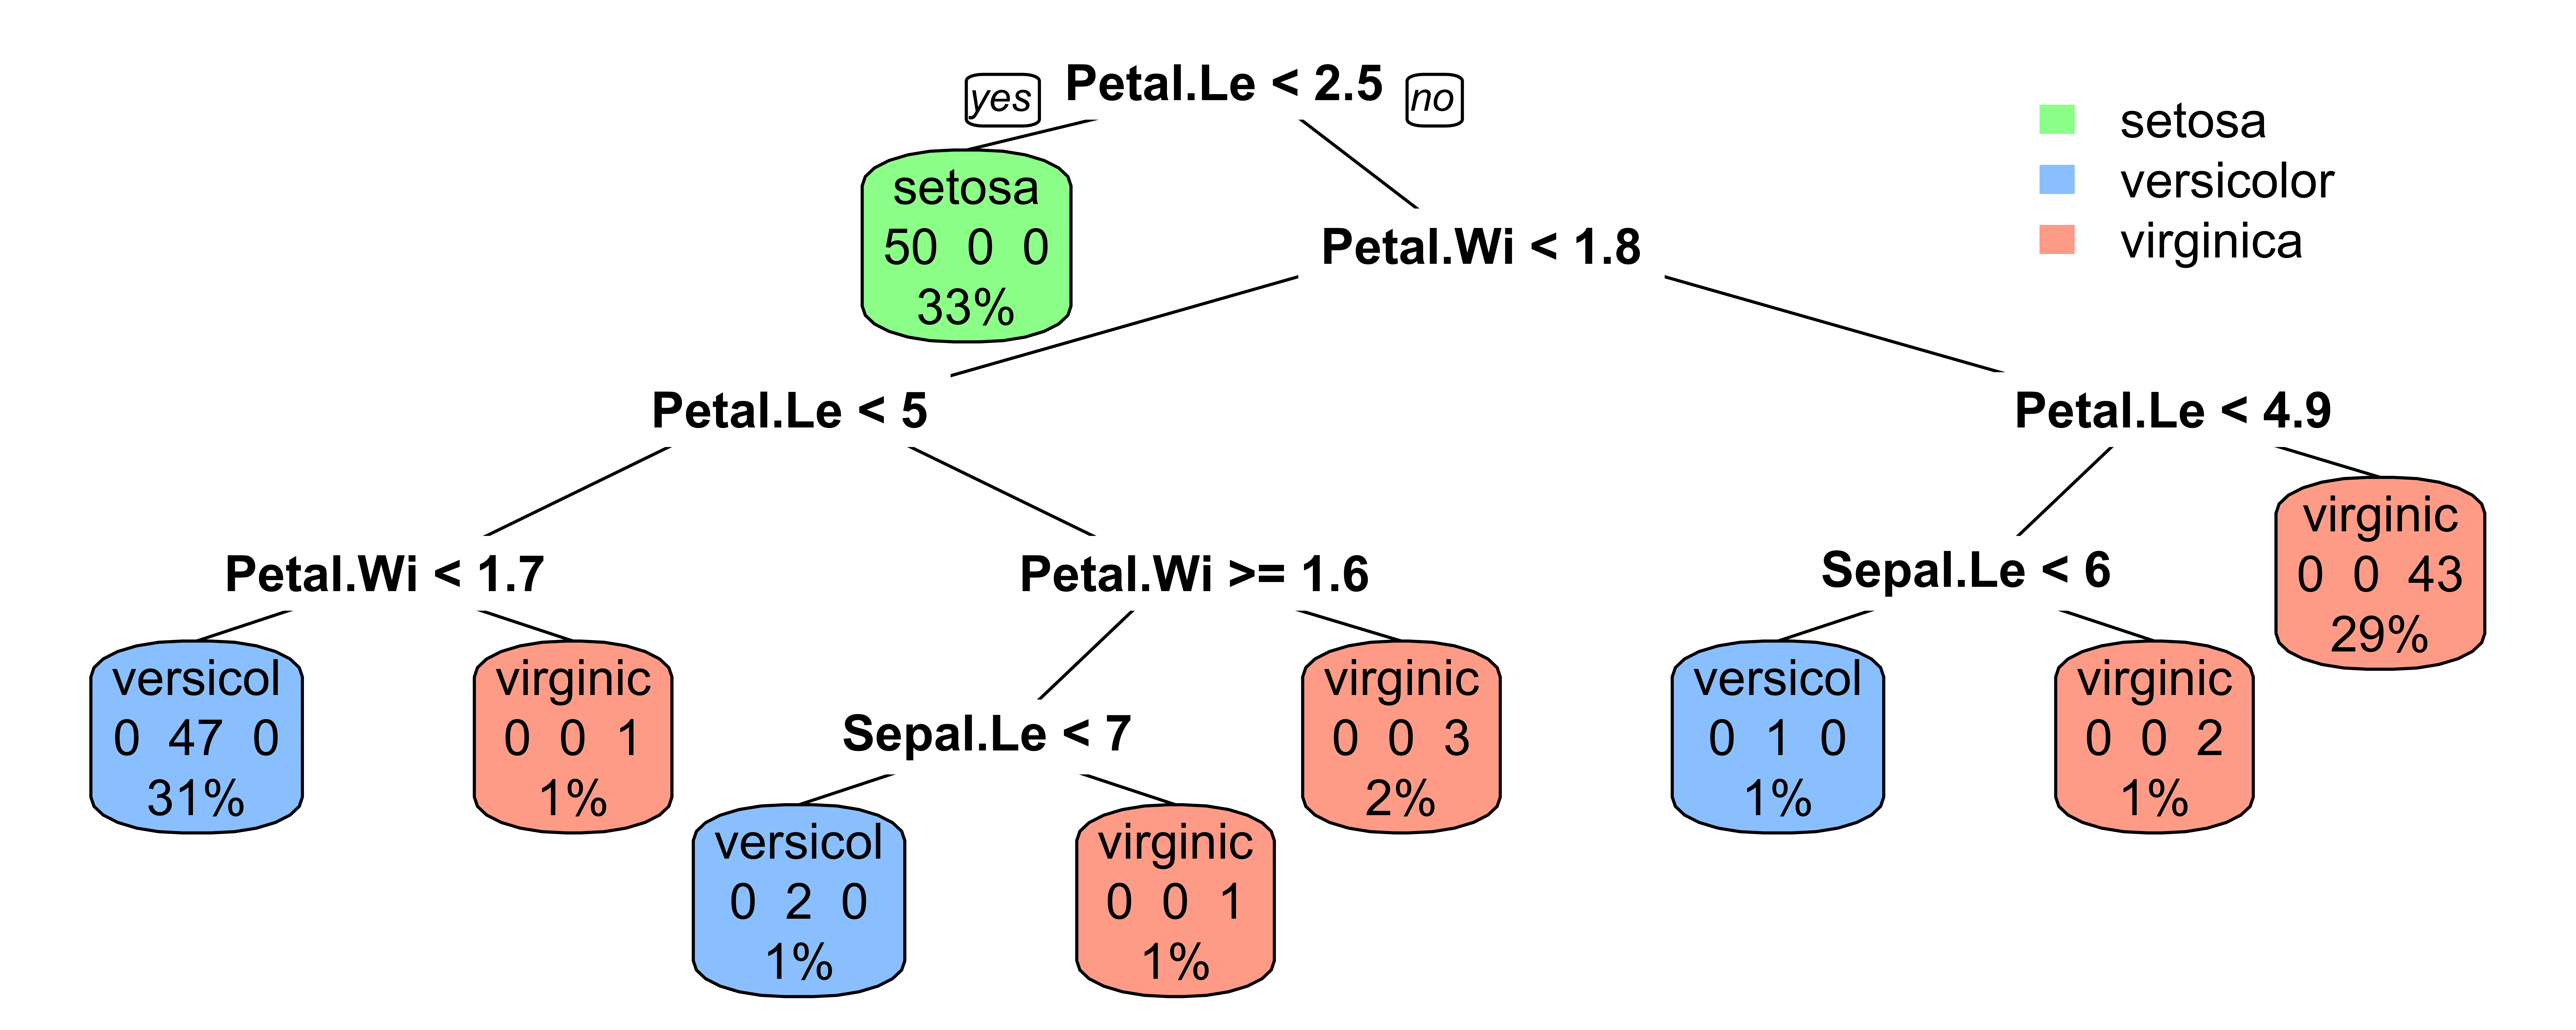
\includegraphics[width=2.5cm,height=3.5cm]{graphics/plot-rpart.png}
	\quad\quad\quad\quad\;\;
	\includegraphics[width=2.5cm,height=3.25cm]{graphics/plot-regression-surface.png}
	\;\;{\color{white}1}
	\end{center}
\end{itemize}


\end{frame}
\normalsize

%%%%%%%%%%
